% Illustrative one-hour interval, with every prompt and review included.
% Each run starts when its prompt is submitted. Review follows B's completion.
% Numeric times below drive the plotted marks and the chronology tests.
\begin{figure}[htp]
\centering
\def\HTWindowStart{0}
\def\HTWindowEnd{60}
\def\HTPromptAStart{0}
\def\HTPromptAEnd{10}
\def\HTPromptBStart{10}
\def\HTPromptBEnd{20}
\def\HTRunAStart{10}
\def\HTRunAEnd{60}
\def\HTRunBStart{20}
\def\HTRunBEnd{40}
\def\HTReviewBStart{40}
\def\HTReviewBEnd{60}
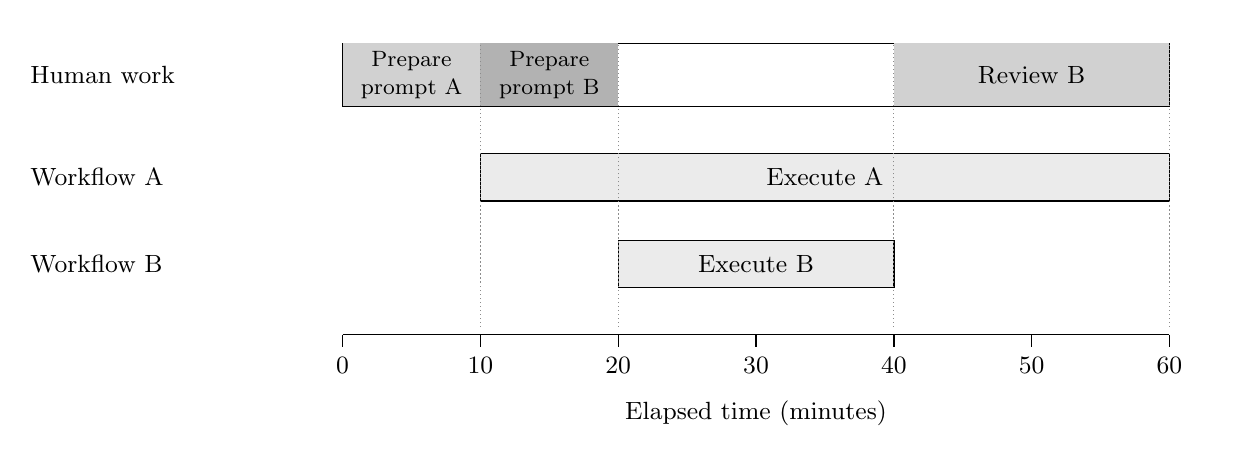
\begin{tikzpicture}[x=1mm,y=1mm,font=\fontsize{9}{11}\selectfont,
  every node/.style={inner sep=1pt,outer sep=0pt}]
  \path[use as bounding box] (0,-8) rectangle (152.4,44);
  \node[anchor=west] at (0,38) {Human work};
  \node[anchor=west] at (0,25) {Workflow A};
  \node[anchor=west] at (0,14) {Workflow B};
  \draw[line width=0.5pt] ({40+1.75*\HTWindowStart},34)
    rectangle ({40+1.75*\HTWindowEnd},42);
  \fill[black!18] ({40+1.75*\HTPromptAStart},34)
    rectangle ({40+1.75*\HTPromptAEnd},42);
  \fill[black!30] ({40+1.75*\HTPromptBStart},34)
    rectangle ({40+1.75*\HTPromptBEnd},42);
  \fill[black!18] ({40+1.75*\HTReviewBStart},34)
    rectangle ({40+1.75*\HTReviewBEnd},42);
  \node[align=center,font=\fontsize{8.5}{10}\selectfont]
    at ({40+1.75*(\HTPromptAStart+\HTPromptAEnd)/2},38) {Prepare\\prompt A};
  \node[align=center,font=\fontsize{8.5}{10}\selectfont]
    at ({40+1.75*(\HTPromptBStart+\HTPromptBEnd)/2},38) {Prepare\\prompt B};
  \node at ({40+1.75*(\HTReviewBStart+\HTReviewBEnd)/2},38) {Review B};
  \draw[fill=black!8,line width=0.5pt] ({40+1.75*\HTRunAStart},22)
    rectangle ({40+1.75*\HTRunAEnd},28);
  \node at ({40+1.75*(\HTRunAStart+\HTRunAEnd)/2},25) {Execute A};
  \draw[fill=black!8,line width=0.5pt] ({40+1.75*\HTRunBStart},11)
    rectangle ({40+1.75*\HTRunBEnd},17);
  \node at ({40+1.75*(\HTRunBStart+\HTRunBEnd)/2},14) {Execute B};
  \foreach \minute in {10,20,40,60} {
    \draw[black!45,densely dotted,line width=0.45pt]
      ({40+1.75*\minute},6) -- ({40+1.75*\minute},42);
  }
  \draw[line width=0.5pt] (40,5) -- (145,5);
  \foreach \minute in {0,10,20,30,40,50,60} {
    \draw[line width=0.5pt] ({40+1.75*\minute},5) -- ({40+1.75*\minute},3.5);
    \node[anchor=north] at ({40+1.75*\minute},2.5) {\minute};
  }
  \node at (92.5,-5) {Elapsed time (minutes)};
\end{tikzpicture}
\caption{\textbf{Human work and automated execution occupy different periods.}
In this illustrative one-hour interval, one person prepares prompt A during minutes 0--10 and prompt B during minutes 10--20, submitting each when preparation ends. Workflow A then executes until minute 60. Workflow B finishes at minute 40, and its result is reviewed during minutes 40--60. The shaded human-work periods total forty minutes, or $2/3$ of a person-hour. The two execution periods total seventy minutes, or $7/6$ workflow-hours, including twenty minutes when both workflows run. The blank human-work period contributes no labour to these tasks.}
\label{fig:human-and-workflow-time}
\end{figure}
